\begin{flushright} {\tiny {\color{gray} (tikz\_elefant\_boundaries.tex)}} \end{flushright}
%~~~~~~~~~~~~~~~~~~~~~~~~~~~~~~~~~~~~~~~~~~~~~~~~~~~~~~~~~~~~~~~~~~~~~~~~~~~~~~~~~~~~~~~~~~~~~~~~~~

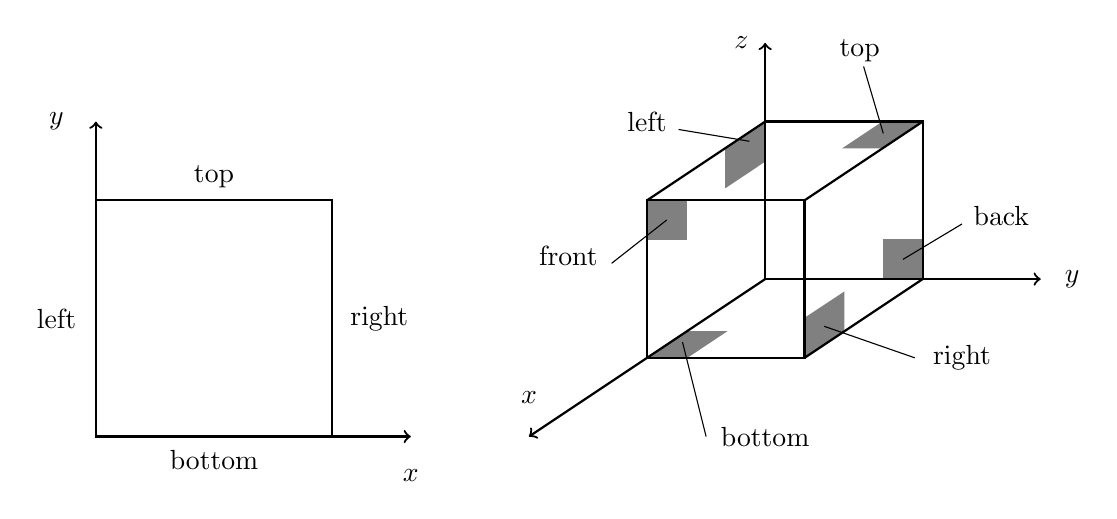
\begin{tikzpicture}
%\draw[step=0.5cm,gray,very thin] (0,0) grid (14,10); %background grid

%2D%%%%%%%%%%%%%%%%%%%%%%%%%%%%%%%%%%%%%%%%%%%%%%%%%%%%%%%%%%%%%%55

\draw[thick] (1,1) -- (4,1) -- (4,4) -- (1,4) -- cycle;  
\draw[thick,->] (1,1)--(5,1);
\draw[thick,->] (1,1)--(1,5);
\node[] at (5,0.5) {$x$};
\node[] at (0.5,5) {$y$};

\node[] at (0.5,2.5) {left};
\node[] at (4.6,2.5) {right};
\node[] at (2.5,0.7) {bottom};
\node[] at (2.5,4.3) {top};

%3d%%%%%%%%%%%%%%%%%%%%%%%%%%%%%%%%%%%%%%%%%%%%%%%%%%%%%%%%%%%%%5

\draw[fill=gray,gray] (8,3.5)--(8.5,3.5)--(8.5,4)--(8,4)--cycle; %front
\draw[fill=gray,gray] (11,3)--(11.5,3)--(11.5,3.5)--(11,3.5)--cycle; %back
\draw[fill=gray,gray] (8,2)--(8.5,2)--(9,2.3333)--(8.5,2.3333)--cycle; %bottom
\draw[fill=gray,gray] (10.5,4.6666)--(11,4.6666)--(11.5,5)--(11,5)--cycle; %top
\draw[fill=gray,gray] (10,2)--(10.5,2.333)--(10.5,2.83)--(10,2.5)--cycle; %right
\draw[fill=gray,gray] (9,4.166)--(9.5,4.5)--(9.5,5)--(9,4.666)--cycle; %left

\draw[thick] (8,2) -- (10,2) -- (10,4) -- (8,4) -- cycle;  
\draw[thick] (9.5,3) -- (11.5,3) -- (11.5,5) -- (9.5,5) -- cycle;  
\draw[thick] (8,4) -- (9.5,5);
\draw[thick] (10,4) -- (11.5,5);
\draw[thick] (10,2) -- (11.5,3);

\draw[thick,->] (9.5,3)--(6.5,1);
\draw[thick,->] (9.5,3)--(9.5,6);
\draw[thick,->] (9.5,3)--(13,3);

\node[] at (8,5) {left};
\node[] at (12,2) {right};
\node[] at (9.5,1) {bottom};
\node[] at (10.7,5.9) {top};
\node[] at (7,3.3) {front};
\node[] at (12.5,3.8) {back};

\node[] at (6.5,1.5) {$x$};
\node[] at (13.4,3) {$y$};
\node[] at (9.2,6) {$z$};

\draw[] (8.75,1)--(8.45,2.2); %bottom
\draw[] (10.25,2.4)--(11.4,2); %right
\draw[] (11.25,3.25)--(12,3.7); %back
\draw[] (10.75,5.7)--(11,4.85); %top
\draw[] (7.55,3.2)--(8.25,3.75); %front
\draw[] (8.4,4.9)--(9.3,4.75); %left

\end{tikzpicture}

